\graphicspath{{Others/}}
\newpage
\section{Déroulement du projet}
\subsection{Organisation théorique du travail}
\subsubsection{Répartition des tâches et prévision de l'emploi du temps}
Le projet fut dès le départ pensé dans le but d'être simple à séparer sous forme de modules, permettant de travailler en parallèle sur plusieurs fonctionnalités.
Comme nous ne maîtrisions pas tous les paramètres (lanage, apprentissage du développement mobile, problèmes techniques), il fut assez difficile de prévoir une charge de travail réaliste associée à chaque module. Nous avons donc estimé 
de manière très grossière le temps de travail par module. Pour être sûrs de pouvoir ajuster le déroulement du projet, nous avons prévu des modules de durées différentes permettant ainsi
de choisir un module en fonction du temps restant, c'est pour cette raison que la durée estimée est supérieure aux 60 heures par personne prévues.
\par
Nous avions estimé, lors de notre premier rendez-vous avec notre tuteur, de travailler 4 heures par semaine de cours et de ne pas travailler les semaines de vacances.
Nous sommes donc parvenus à finaliser l'emploi du temps suivant, qui n'avait pas pour but d'être suivi à la lettre.
\vfill
\begin{figure}[!h]
    \begin{center}
        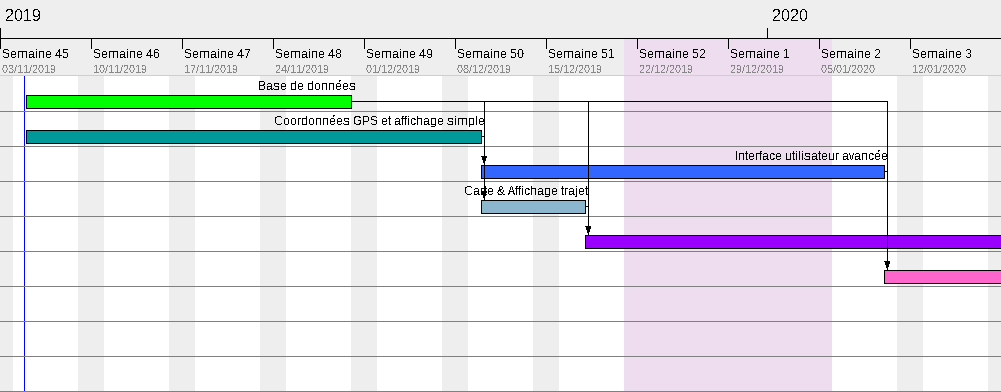
\includegraphics[height=6cm]{test-1.png}
        \caption{Première partie du diagramme de Gantt prévisionnel}
    \end{center}
\end{figure}
\subsubsection{Explications sur les tâches}
Les deux premiers objectifs fixés étaient assez simples, leur but étaient de nous laisser le temps d'être à l'aise avec les technologies choisies.
Nous devions prévoir la base de données, c'est à dire la concevoir et la mettre en place sur la machine virtuelle. En parallèle de cela, nous devions réussir à récupérer les coordonnées GPS du téléphone, et réussir à les afficher.
\par
Les objectifs suivants étaient d'enrichir l'expérience utilisateur en améliorant l'interface. Nous voulions en premier permettre la gestion d'un compte utilisateur depuis l'application, ce qui implique un écran de connexion, un écran de création de comptes ainsi qu'un écran de gestion de comptes.
Dans un second point (développé en parallèle) nous devions enrichir l'interface fonctionnelle de l'application, c'est à dire insérer une interface contenant une carte sur laquelle notre trajet serait affichable (cela sous entend de stocker les coordonnées aquises).
\par
Nous avions prévu de faire évoluer l'application en rajoutant du contenu. Il aurait fallu ajouter des statistiques plus complètes sur les trajets effectués, comme par exemple$\ :$ le dénivelé, la météo ou bien une estimation des calories dépensées.
Il fallait également introduire une gestion des utilisateurs plus développée, qui permettrait de gérer plus finement les droits d'accès. On aurait ainsi pu dire qu'un autre utilisateur avait participé à un trajet, ou bien qu'il avait le droit d'en modifier le contenu.
De la même manière, on aurait pu créer des groupes d'utilisateurs pour un club par exemple. Dans ces groupes tout le monde aurait accès en lecture uniquement sauf les administrateurs. Ainsi un club sportif aurait pu utiliser l'application pour organiser des séances de randonnées.
\par
Un des derniers points à mettre en place était l'affichage des statistiques précédemments acquises sous la forme de graphique où l'on aurait pu choisir l'échelle, et les trajets qui rentraient en compte.
Le dernier point était radicalement plus difficile à traiter, nous voulions finir le développement de l'application en la faisant se rapprocher d'un réseau social. On aurait alors pu avoir des amis, un fil d'actualité contenant les trajets (publics) de nos amis. On aurait aussi pu partager
nos trajets via des liens webs, qui auraient été ouvrables uniquement par notre application.
\par
Enfin il y avait la dernière tâche évidente, la rédaction du rapport. Nous avions prévu de prendre des notes au fur et à mesure du développement du projet pour parvenir à rédiger le rapport plus efficacement.
\vfill
\begin{figure}[!h]
    \begin{center}
        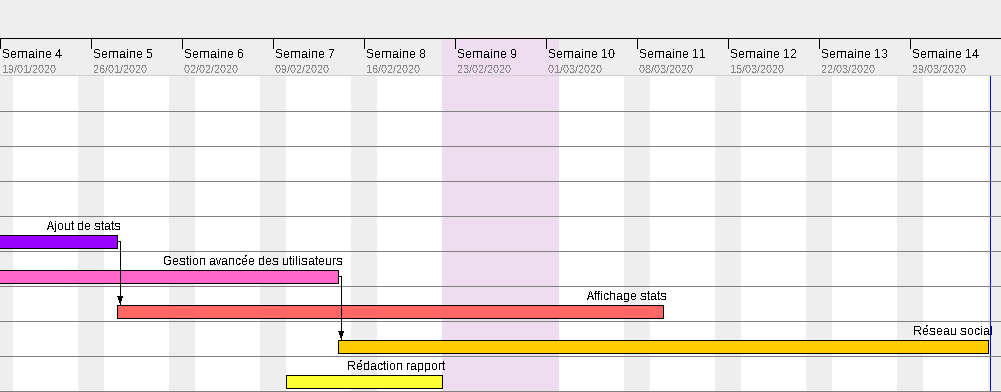
\includegraphics[height=6cm]{test-2.png}
        \caption{Seconde partie du diagramme de Gantt prévisionnel}
    \end{center}
\end{figure}






\subsection{Organisation réelle du travail}
\subsubsection{Répartion des tâches et emploi du temps}
Au lieu de débuter le projet comme prévu$\ :\ $chacun sur un module, nous avons préféré faire quelques séances de travail en commun afin de découvrir ensemble l'environnement android, et de nous mettre entièrement d'accord sur la suite.
\par
Nous avons ensuite séparé le travail, un s'est chargé du développement android et l'autre de la base de données. Développer sous android implique nécessairement d'en étudier plus le fonctionnement. D'autant plus que nous voulions utiliser Kotlin qui est un langage que nous ne connaissions pas du tout.
Pour la base de données le plus difficile était d'en faire l'installation et la configuration.
\par
Nous avons été assez surpris par la charge de travail à fournir sur deux semaines du fait des partiels qui ont suivis. En plus nous avons eu plusieurs travaux pratiques importants à rendre la semaine suivante.
Nous nous sommes replongés dans le travail la semaine précédant les vacances. Nous avons eu le temps d'intégrer l'interface finale de l'application avec le menu sur le côté gauche. Et nous avons commencé le développement du serveur qui allait interagir avec la base de données.
\par
Ensuite nous avons eu un problème technique lié à la période des vacances que nous détaillons dans la partie "Problèmes rencontrés". Puis nous avons commencé à développer la communication entre le serveur et l'application ainsi que l'affichage d'un trajet sur une carte. Un second problème est survenu ce qui nous a imposé de mettre en pause le développement du serveur, pour finalement ne jamais le reprendre.
Nous avons donc commencé le rapport. L'application s'est étoffée pour fournir l'enregistrement de trajets en local, ainsi que leur sauvegarde (sur le téléphone) sous la forme d'un historique (accessible depuis l'application).
Ces dernières fonctionnalités étant fournies par une bibliothèque de gestion de nos structures de données.
\par
Enfin nous avons dû arrêter le développement de l'application pour nous concentrer sur l'écriture du rapport de projet.
\vfill
\begin{figure}[!h]
    \begin{center}
        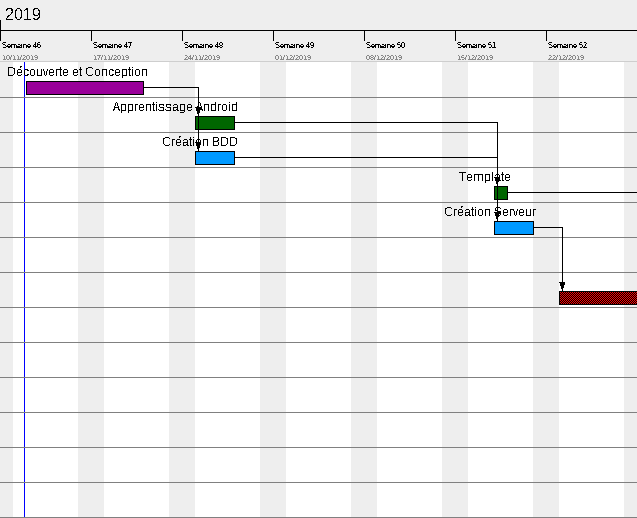
\includegraphics[height=8cm]{reel-1.png}
        \caption{Première partie du diagramme de Gantt réel}
    \end{center}
\end{figure}
\newpage
\subsubsection{Méthodologie de travail}
Nous avons essayé autant que possible de nous organiser à l'avance sur le travail. C'est à dire qu'en fin de chaque séance nous avons essayé de fixer un objectif à réaliser à la séance suivante.
Pendant le deuxième semestre, nous avons travaillé plus souvent séparément du fait de nos emplois du temps scolaires. Nous parlions alors régulièrement de notre avancement respectif en se donnant une date limite pour chaque tâche.
\par
Lors du développement de la bibliothèque de gestion des trajets, nous avons naturellement mis en place une méthode de travail agile, sous la forme d'itérations. Ainsi lorsqu'une fonctionnalité de l'application avait besoin d'un accès à la structure de données, cette partie de la bibliothèque était développée.
Cela nous a permis de travailler efficacement, en mettant le doigt rapidement sur ce qui ne convenait pas à l'application.
\par
Pour ce qui est de la communication avec notre tuteur, nous devions envoyer des mails toutes les semaines pour qu'il puisse suivre l'avancement du projet. Dans la pratique, nous avons été moins réguliers. Nous avons cependant gardé le contact au fur et à mesure des évolutions, ainsi que lorsque nous avions des difficultés.
\vfill
\begin{figure}[!h]
    \begin{center}
        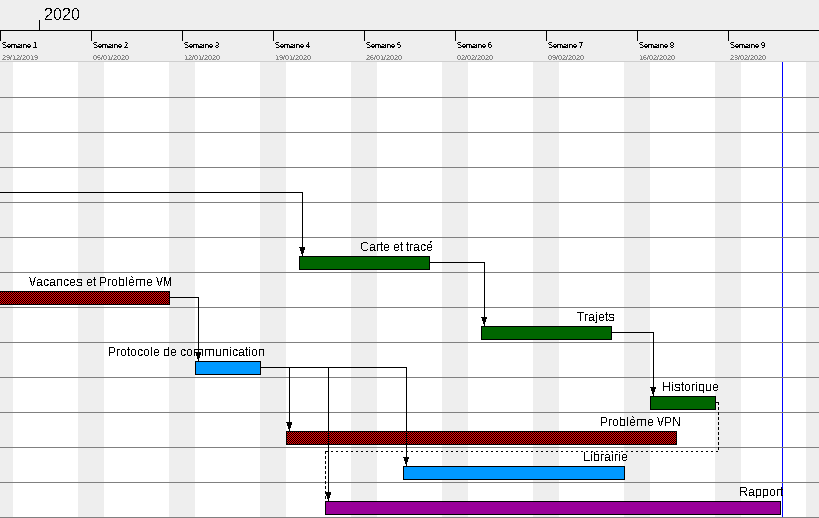
\includegraphics[height=8cm]{reel-2.png}
        \caption{Seconde partie du diagramme de Gantt réel}
    \end{center}
\end{figure}
\newpage




\subsection{Problèmes rencontrés}
\subsubsection{Langage Kotlin}
Lors de ce projet nous avons rencontré plusieurs problèmes majeurs qui nous ont obligés à changer l'orientation du projet.
Le premier problème était lié au langage, nous avions prévu de développer l'application en utilisant le langage Kotlin, qui est le nouveau langage officiel.
C'est un langage qui semble très intéressant avec son paradigme fonctionnel. Cependant, nous n'avions également que très peu d'expérience
dans le développement mobile qui est aussi très riche avec beaucoup d'aspects et fonctionnements propres à apprendre. Il s'est très vite révélé
qu'il était très difficile d'avancer le projet en apprenant en parallèle le développement mobile et le Kotlin. De plus, lorsqu'un problème
survient, il est beaucoup plus aisé de trouver de la documentation ou de l'aide avec le langage Java puisque le Kotlin est beaucoup plus récent.
Il a donc été convenu de reprendre le projet avec le langage Java afin de se concentrer sur l'apprentissage du développement mobile.
\subsubsection{Machine virtuelle}
Nous avons ensuite eu des problèmes liés au matériel indépendants de notre volonté.
Pendant les vacances de Noël, nous n'avons pas pu avancer autant que nécessaire, car la machine virtuelle que nous avait fournie l'ISIMA ne fonctionnait pas.
Nous avons donc passé plusieurs jours à essayer de trouver où était notre erreur de configuration, avant de se rendre compte que la machine virtuelle, lors d'une maintenance, avait était éteinte mais pas rallumée.
\subsubsection{Réseau}
Enfin le problème qui nous a le plus bloqué est survenu lorsque nous avons voulu connecter l'application au serveur. En effet, pour accéder à la machine virtuelle il faut obligatoirement être connecté au réseau privé de l'ISIMA.
Pour cela l'ISIMA fournit un fichier de configuration pour le logiciel OpenVPN. Cette configuration fonctionne parfaitement sur ordinateur. Cependant lorsque nous l'avons mise sur nos téléphones, nous perdions tout accès à internet.
Nous avons ensuite contacté le service informatique de l'école, qui a accepté de prendre un rendez-vous pour essayer de diagnostiquer plus précisémment le problème. Nous avons lors de ce rendez-vous, réussi à confirmer que le problème venait
du fichier de configuration qui utilisait un paramètre de compression des données non-compatible avec la version android du logiciel. Nous avons ensuite essayé de trouver des solutions pour pouvoir continuer le projet.
Une fois les délibérations terminées, il a été conclu que nous n'aurions pas de solution dans les délais qui nous étaient imposés. Nous avons donc arrêter le développement de la partie réseau et serveur pour nous concentrer sur un stockage local des informations.
